\chapter{Text, Data, And Tokenization For TinyGPT}

The first two chapters showed the TinyGPT pipeline and the math tools behind it. This chapter focuses on the beginning of the pipeline: how raw text becomes token IDs, how token IDs become training examples, and how software should store those examples for reproducible training.

The central lesson is simple:

\begin{quote}
A GPT model does not train on text. It trains on integer token sequences created by a tokenizer.
\end{quote}

\section{Chapter Goals}

By the end of this chapter, you should be able to:

\begin{itemize}
  \item explain why text must be converted into token IDs;
  \item compare character, word, and subword tokenization;
  \item trace the TinyGPT corpus into a vocabulary and token stream;
  \item explain Byte Pair Encoding with a concrete merge example;
  \item construct input-target windows from a token stream;
  \item write the code logic for \texttt{encode}, \texttt{decode}, \texttt{get\_batch}, and binary token storage;
  \item describe the data-quality checks needed before training.
\end{itemize}

\section{The TinyGPT Corpus}

We keep the same small teaching corpus:

\begin{lstlisting}
MapleAI trains Tiny GPT models .
Tiny GPT models learn from tokens .
Tokens become vectors .
Vectors flow through attention .
\end{lstlisting}

This corpus is intentionally small. It lets us inspect every token. A real training corpus may contain billions of tokens, but the logic is the same.

\begin{center}
\begin{tikzpicture}[
  box/.style={draw, rounded corners=2pt, minimum height=0.7cm, text width=2.6cm, align=center},
  arrow/.style={-{Latex[length=2mm]}, thick}
]
\node[box, fill=blue!5] (docs) at (0,0) {text documents};
\node[box, fill=blue!5] (clean) at (3.0,0) {clean and normalize};
\node[box, fill=blue!5] (tok) at (6.0,0) {tokenizer};
\node[box, fill=red!8] (ids) at (9.0,0) {token ID stream};
\node[box, fill=red!8] (batches) at (6.0,-1.3) {training batches};
\node[box, fill=red!8] (model) at (3.0,-1.3) {TinyGPT};
\draw[arrow] (docs) -- (clean);
\draw[arrow] (clean) -- (tok);
\draw[arrow] (tok) -- (ids);
\draw[arrow] (ids) |- (batches);
\draw[arrow] (batches) -- (model);
\end{tikzpicture}
\end{center}

\section{Who Manages The Data?}

Data is not one thing. A training system manages a chain of artifacts. Each artifact has a different owner, format, and correctness check.

\begin{center}
\begin{tikzpicture}[
  box/.style={draw, rounded corners=2pt, minimum height=0.72cm, text width=2.35cm, align=center},
  arrow/.style={-{Latex[length=2mm]}, thick},
  lab/.style={font=\small, align=center}
]
\node[box, fill=blue!5] (raw) at (0,0) {raw text\\human-readable};
\node[box, fill=blue!5] (clean) at (2.9,0) {clean text\\normalized};
\node[box, fill=blue!5] (tok) at (5.8,0) {tokenizer\\vocab + rules};
\node[box, fill=red!8] (ids) at (8.7,0) {token stream\\integer IDs};
\node[box, fill=red!8] (bin) at (8.7,-1.45) {binary files\\\texttt{train.bin}};
\node[box, fill=gray!12] (meta) at (5.8,-1.45) {metadata\\JSON};
\node[box, fill=gray!12] (batch) at (2.9,-1.45) {batch tensors\\\(x,y\)};
\node[box, fill=gray!12] (model) at (0,-1.45) {model input\\training step};
\draw[arrow] (raw) -- (clean);
\draw[arrow] (clean) -- (tok);
\draw[arrow] (tok) -- (ids);
\draw[arrow] (ids) -- (bin);
\draw[arrow] (ids) -- (meta);
\draw[arrow] (bin) -- (batch);
\draw[arrow] (meta) -- (batch);
\draw[arrow] (batch) -- (model);
\node[lab] at (4.3,-2.35) {The model never sees raw text. It sees batches made from stored token IDs plus tokenizer metadata.};
\end{tikzpicture}
\end{center}

\begin{longtable}{p{0.2\textwidth}p{0.25\textwidth}p{0.39\textwidth}}
\toprule
\term{Artifact} & \term{Managed by} & \term{Correctness question} \\
\midrule
Raw text & data curator & Is it allowed, useful, and safe? \\
Clean text & preprocessing script & Did normalization preserve meaning? \\
Tokenizer & tokenizer trainer/designer & Are encode/decode stable and saved? \\
Token stream & prepare script & Do IDs match the tokenizer? \\
Binary file & storage pipeline & Is dtype/count/checksum correct? \\
Batch \(x,y\) & data loader & Is the target shifted by exactly one? \\
Training sample & model/trainer & Does loss compare logits to the right targets? \\
\bottomrule
\end{longtable}

This management view prevents a common beginner mistake: thinking tokenization is a quick preprocessing detail. In reality, the tokenizer and token files are part of the model's identity.

\section{Why Text Needs Tokenization}

Computers can store text as bytes or Unicode characters, but a neural network needs tensors of numbers. The model needs a finite vocabulary:

\[
\mathcal{V} = \{0,1,\ldots,V-1\}.
\]

For TinyGPT, \(V=9\):

\begin{longtable}{p{0.24\textwidth}p{0.24\textwidth}p{0.34\textwidth}}
\toprule
\term{Token} & \term{ID} & \term{Role in sample corpus} \\
\midrule
\texttt{MapleAI} & 0 & organization token \\
\texttt{trains} & 1 & verb \\
\texttt{Tiny} & 2 & adjective/name token \\
\texttt{GPT} & 3 & model-family token \\
\texttt{models} & 4 & noun \\
\texttt{learn} & 5 & verb \\
\texttt{from} & 6 & preposition \\
\texttt{tokens} & 7 & noun \\
\texttt{.} & 8 & punctuation \\
\bottomrule
\end{longtable}

The token ID is an index. It points into the embedding table:

\[
E_{\text{tok}}\in\mathbb{R}^{V\times C}.
\]

With \(V=9\) and \(C=6\), TinyGPT uses:

\[
E_{\text{tok}}\in\mathbb{R}^{9\times6}.
\]

\begin{center}
\begin{tikzpicture}[
  cell/.style={draw, minimum width=0.8cm, minimum height=0.5cm, align=center},
  lab/.style={font=\small, align=center},
  arrow/.style={-{Latex[length=2mm]}, thick}
]
\node[cell, fill=blue!5] (id) at (0,0) {ID 2};
\node[lab] at (0,-0.65) {\texttt{Tiny}};
\draw[arrow] (id) -- (1.2,0);
\foreach \r in {0,1,2,3,4,5,6,7,8} {
  \foreach \c in {0,1,2,3,4,5} {
    \ifnum\r=2
      \node[cell, fill=red!8, minimum width=0.38cm] at (1.8+\c*0.4,-\r*0.28+1.1) {};
    \else
      \node[cell, fill=gray!10, minimum width=0.38cm] at (1.8+\c*0.4,-\r*0.28+1.1) {};
    \fi
  }
}
\node[lab] at (3.0,-1.85) {embedding table\\\shape{[9,6]}};
\node[lab, text=maplered] at (5.1,0.55) {row 2 becomes\\a 6-number vector};
\draw[arrow, maplered] (4.25,0.54) -- (3.9,0.54);
\end{tikzpicture}
\end{center}

\term{Why this matters}: if the tokenizer changes, token ID \(2\) may no longer mean \texttt{Tiny}. Then the model's embedding row 2 would be interpreted incorrectly. This is why tokenizer identity is part of every serious checkpoint contract.

\section{A Token's Life Cycle}

The token \texttt{Tiny} appears simple to a reader, but the training system manages it through several representations.

\begin{center}
\begin{tikzpicture}[
  box/.style={draw, rounded corners=2pt, minimum height=0.72cm, text width=2.1cm, align=center},
  arrow/.style={-{Latex[length=2mm]}, thick},
  lab/.style={font=\small, align=center}
]
\node[box, fill=blue!5] (text) at (0,0) {raw text\\\texttt{Tiny}};
\node[box, fill=blue!5] (token) at (2.7,0) {token string\\\texttt{Tiny}};
\node[box, fill=blue!5] (id) at (5.4,0) {token ID\\2};
\node[box, fill=red!8] (bin) at (8.1,0) {stored bytes\\\texttt{02 00}};
\node[box, fill=red!8] (tensor) at (8.1,-1.35) {batch tensor\\cell in \(x\)};
\node[box, fill=gray!12] (embed) at (5.4,-1.35) {embedding row\\\(E_{\text{tok}}[2]\)};
\node[box, fill=gray!12] (model) at (2.7,-1.35) {model vector\\part of \(X\)};
\draw[arrow] (text) -- (token);
\draw[arrow] (token) -- (id);
\draw[arrow] (id) -- (bin);
\draw[arrow] (bin) -- (tensor);
\draw[arrow] (tensor) -- (embed);
\draw[arrow] (embed) -- (model);
\node[lab] at (4.1,-2.25) {The same token moves from human text to bytes to tensor cell to learned vector.};
\end{tikzpicture}
\end{center}

This life cycle explains why tokenizer bugs are expensive. If \texttt{Tiny} maps to the wrong ID, every later stage uses the wrong embedding row and the model learns from corrupted examples.

\section{Tokenizer Levels}

There are three useful ways to split text.

\subsection{Character-Level Tokenization}

Character tokenization splits text into characters:

\begin{quote}
\texttt{Tiny} \(\rightarrow\) \texttt{T}, \texttt{i}, \texttt{n}, \texttt{y}
\end{quote}

\begin{center}
\begin{tikzpicture}[
  cell/.style={draw, minimum width=0.8cm, minimum height=0.55cm, align=center},
  arrow/.style={-{Latex[length=2mm]}, thick}
]
\node at (-1.0,0) {\texttt{Tiny}};
\draw[arrow] (-0.45,0) -- (0.05,0);
\foreach \i/\ch in {0/T,1/i,2/n,3/y} {
  \node[cell, fill=blue!5] at (\i*0.9+0.5,0) {\texttt{\ch}};
}
\end{tikzpicture}
\end{center}

\term{Strength}: very simple and handles unseen words.  
\term{Weakness}: sequences become long, so attention becomes expensive.

\subsection{Word-Level Tokenization}

Word tokenization splits text into words and punctuation:

\begin{quote}
\texttt{Tiny GPT models .} \(\rightarrow\)
\texttt{Tiny}, \texttt{GPT}, \texttt{models}, \texttt{.}
\end{quote}

This is the easiest tokenizer for our first chapters. Its weakness is that rare or unseen words are hard to handle. If the vocabulary does not contain \texttt{Transformer}, what ID should it receive?

\subsection{Subword Tokenization}

Subword tokenization splits rare words into smaller known pieces:

\begin{quote}
\texttt{tokenization} \(\rightarrow\) \texttt{token}, \texttt{ization}
\end{quote}

or, depending on the learned tokenizer:

\begin{quote}
\texttt{tokenization} \(\rightarrow\) \texttt{tok}, \texttt{en}, \texttt{ization}
\end{quote}

Subword tokenization is the common practical choice for modern LLMs because it balances sequence length and open-vocabulary behavior.

\begin{longtable}{p{0.22\textwidth}p{0.28\textwidth}p{0.32\textwidth}}
\toprule
\term{Level} & \term{Good for} & \term{Tradeoff} \\
\midrule
Character & simple demos, robustness & long sequences \\
Word & intuition, small controlled corpora & unknown words \\
Subword & practical LLM training & tokenizer training complexity \\
\bottomrule
\end{longtable}

\section{Byte Pair Encoding By Example}

Byte Pair Encoding, or BPE, learns subword tokens by repeatedly merging frequent adjacent pairs. We will use a tiny visual example.

Suppose the corpus has these word pieces:

\begin{lstlisting}
l o w
l o w
l o w e r
n e w
w i d e r
\end{lstlisting}

The pair \texttt{l o} appears often, so BPE may merge it:

\begin{center}
\begin{tikzpicture}[
  cell/.style={draw, minimum width=0.55cm, minimum height=0.5cm, align=center},
  arrow/.style={-{Latex[length=2mm]}, thick},
  lab/.style={font=\small, align=center}
]
\node[lab] at (1.0,0.7) {before};
\foreach \i/\ch in {0/l,1/o,2/w} {
  \node[cell, fill=blue!5] at (\i*0.65,0) {\texttt{\ch}};
}
\draw[arrow] (2.4,0) -- (3.2,0);
\node[lab] at (4.1,0.7) {after merge};
\node[cell, fill=red!8, minimum width=0.9cm] at (3.8,0) {\texttt{lo}};
\node[cell, fill=blue!5] at (4.7,0) {\texttt{w}};
\node[lab] at (2.75,-0.7) {merge frequent pair \texttt{l o}};
\end{tikzpicture}
\end{center}

Later, \texttt{lo} and \texttt{w} may merge into \texttt{low}. BPE gradually builds a vocabulary of useful pieces.

\begin{lstlisting}
start:    l o w
merge 1:  lo w
merge 2:  low
\end{lstlisting}

\term{Why BPE works}: common sequences become short tokens, while rare words can still be represented as smaller pieces. This keeps the vocabulary finite without making all sequences character-level long.

\section{Tokenizer Source Code Logic}

For TinyGPT, a word-level tokenizer is enough. A minimal implementation has four responsibilities:

\begin{enumerate}
  \item normalize text;
  \item split text into tokens;
  \item map tokens to IDs;
  \item map IDs back to tokens.
\end{enumerate}

\subsection{Normalize And Split}

\begin{lstlisting}[language=Python]
def normalize(text):
    text = text.replace(".", " .")
    text = " ".join(text.split())
    return text

def split_tokens(text):
    return normalize(text).split()
\end{lstlisting}

\term{Why this exists}: punctuation must be handled consistently. If one line contains \texttt{tokens.} and another contains \texttt{tokens .}, a word tokenizer may treat them differently unless we normalize.

\subsection{Build Vocabulary}

\begin{lstlisting}[language=Python]
def build_vocab(texts):
    tokens = []
    for text in texts:
        tokens.extend(split_tokens(text))
    unique = sorted(set(tokens))
    token_to_id = {tok: i for i, tok in enumerate(unique)}
    id_to_token = {i: tok for tok, i in token_to_id.items()}
    return token_to_id, id_to_token
\end{lstlisting}

For teaching, we manually keep the Chapter 1 order. In a real tokenizer, vocabulary order must be saved exactly.

\subsection{Encode And Decode}

\begin{lstlisting}[language=Python]
def encode(text, token_to_id):
    return [token_to_id[tok] for tok in split_tokens(text)]

def decode(ids, id_to_token):
    return " ".join(id_to_token[i] for i in ids)
\end{lstlisting}

\term{Round-trip test}:

\begin{lstlisting}[language=Python]
text = "Tiny GPT models learn from tokens."
ids = encode(text, token_to_id)
decoded = decode(ids, id_to_token)
print(ids)
print(decoded)
\end{lstlisting}

Expected IDs:

\[
[2,3,4,5,6,7,8].
\]

Expected decoded text:

\begin{quote}
\texttt{Tiny GPT models learn from tokens .}
\end{quote}

The spacing before punctuation is acceptable for this toy tokenizer. A production tokenizer should define exactly how text is reconstructed.

\section{From Documents To One Token Stream}

For next-token prediction, a corpus becomes a long sequence:

\[
s=[s_1,s_2,\ldots,s_N].
\]

Using the TinyGPT corpus, a simplified stream is:

\[
[0,1,2,3,4,8,2,3,4,5,6,7,8,\ldots].
\]

\begin{center}
\begin{tikzpicture}[
  cell/.style={draw, minimum width=0.65cm, minimum height=0.5cm, align=center},
  lab/.style={font=\small, align=center},
  arrow/.style={-{Latex[length=2mm]}, thick}
]
\node[lab] at (1.3,0.75) {document 1};
\foreach \i/\v in {0/0,1/1,2/2,3/3,4/4,5/8} {
  \node[cell, fill=blue!5] at (\i*0.7,0) {\v};
}
\node[lab] at (6.1,0.75) {document 2};
\foreach \i/\v in {0/2,1/3,2/4,3/5,4/6,5/7,6/8} {
  \node[cell, fill=red!8] at (4.4+\i*0.7,0) {\v};
}
\draw[arrow] (9.8,0) -- (10.6,0);
\node[lab] at (11.8,0) {more tokens};
\node[lab] at (5.1,-0.8) {concatenate documents into one training stream};
\end{tikzpicture}
\end{center}

Some systems insert a special end-of-document token. TinyGPT's toy vocabulary does not include one yet, but larger training systems usually should.

\section{Train, Validation, And Test Splits}

The data must be split before training. A typical split is:

\begin{itemize}
  \item training tokens: used to update weights;
  \item validation tokens: used to monitor training decisions;
  \item test tokens: used for final reporting.
\end{itemize}

\begin{center}
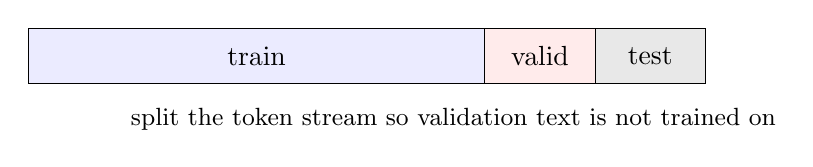
\begin{tikzpicture}[
  seg/.style={draw, minimum height=0.7cm, align=center},
  lab/.style={font=\small}
]
\node[seg, fill=blue!8, minimum width=5.8cm] at (0,0) {train};
\node[seg, fill=red!8, minimum width=1.4cm] at (3.6,0) {valid};
\node[seg, fill=gray!18, minimum width=1.4cm] at (5.0,0) {test};
\node[lab] at (2.5,-0.8) {split the token stream so validation text is not trained on};
\end{tikzpicture}
\end{center}

\term{Why this matters}: if validation examples appear in training, validation loss becomes misleadingly good. This is called leakage.

\section{Training Windows}

Given the stream:

\[
s=[2,3,4,5,6,7,8],
\]

and \(T=4\), a training window starting at index 0 uses:

\[
\text{chunk}=[2,3,4,5,6].
\]

Then:

\[
x=[2,3,4,5],
\qquad
y=[3,4,5,6].
\]

\begin{center}
\begin{tikzpicture}[
  cell/.style={draw, minimum width=0.7cm, minimum height=0.5cm, align=center},
  lab/.style={font=\small, align=center},
  arrow/.style={-{Latex[length=2mm]}, thick}
]
\node[lab] at (-0.7,0) {stream};
\foreach \i/\v in {0/2,1/3,2/4,3/5,4/6,5/7,6/8} {
  \node[cell, fill=gray!10] at (\i*0.78,0) {\v};
}
\draw[red, very thick] (-0.38,0.35) rectangle (3.5,-0.35);
\node[lab, text=red!70!black] at (1.55,0.82) {\(T+1=5\) tokens needed};
\foreach \i/\v in {0/2,1/3,2/4,3/5} {
  \node[cell, fill=blue!6] at (\i*0.78,-1.1) {\v};
}
\node[lab] at (-0.7,-1.1) {\(x\)};
\foreach \i/\v in {0/3,1/4,2/5,3/6} {
  \node[cell, fill=red!8] at (\i*0.78,-1.85) {\v};
}
\node[lab] at (-0.7,-1.85) {\(y\)};
\draw[arrow] (0,-0.3) -- (0,-0.82);
\draw[arrow] (0.78,-0.3) -- (0,-1.58);
\end{tikzpicture}
\end{center}

This is the same shift used in Chapters 1 and 2. The dataset reader's job is to produce many such windows.

\section{Batch Construction}

A batch is several windows stacked together:

\[
X\in\mathbb{Z}^{B\times T},
\qquad
Y\in\mathbb{Z}^{B\times T}.
\]

For \(B=2\) and \(T=4\):

\[
X=
\begin{bmatrix}
2&3&4&5\\
0&1&2&3
\end{bmatrix},
\qquad
Y=
\begin{bmatrix}
3&4&5&6\\
1&2&3&4
\end{bmatrix}.
\]

\begin{center}
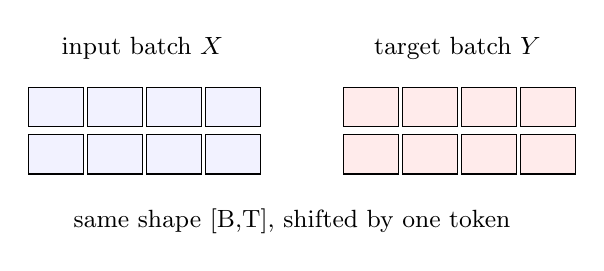
\begin{tikzpicture}[
  cell/.style={draw, minimum width=0.7cm, minimum height=0.5cm, align=center},
  lab/.style={font=\small, align=center}
]
\node[lab] at (1.1,0.75) {input batch \(X\)};
\foreach \r/\vals in {0/{2,3,4,5},1/{0,1,2,3}} {
  \foreach \c in {0,1,2,3} {
    \node[cell, fill=blue!5] at (\c*0.75,-\r*0.6) {};
  }
}
\node[lab] at (5.1,0.75) {target batch \(Y\)};
\foreach \r/\vals in {0/{3,4,5,6},1/{1,2,3,4}} {
  \foreach \c in {0,1,2,3} {
    \node[cell, fill=red!8] at (4+\c*0.75,-\r*0.6) {};
  }
}
\node[lab] at (3.0,-1.45) {same shape \shape{[B,T]}, shifted by one token};
\end{tikzpicture}
\end{center}

\section{Batch Source Code Logic}

\begin{lstlisting}[language=Python]
def get_batch(tokens, batch_size, block_size):
    # tokens is a 1D tensor or list of token IDs.
    starts = torch.randint(
        low=0,
        high=len(tokens) - block_size - 1,
        size=(batch_size,),
    )

    xs = []
    ys = []
    for i in starts:
        chunk = tokens[i : i + block_size + 1]
        xs.append(chunk[:-1])
        ys.append(chunk[1:])

    x = torch.stack(xs)  # [B, T]
    y = torch.stack(ys)  # [B, T]
    return x, y
\end{lstlisting}

\term{Function by function}:

\begin{itemize}
  \item \texttt{torch.randint}: chooses random starting positions.
  \item \texttt{chunk}: grabs \(T+1\) consecutive tokens.
  \item \texttt{chunk[:-1]}: creates the input row.
  \item \texttt{chunk[1:]}: creates the target row.
  \item \texttt{torch.stack}: turns a list of rows into a batch tensor.
\end{itemize}

\term{Why the upper bound subtracts \texttt{block\_size + 1}}: each start position must have enough future tokens to build both \(x\) and \(y\). Otherwise the target row would be too short.

\section{Binary Token Files}

Large token streams are usually stored as binary arrays. Text files are easy to inspect but slower and larger. A simple training-pack layout is:

\begin{lstlisting}
data/tokens/tinygpt/
  train.bin
  train.meta.json
  valid.bin
  valid.meta.json
\end{lstlisting}

For TinyGPT, token IDs fit in \texttt{uint16}. Larger vocabularies may require \texttt{uint32}.

\begin{center}
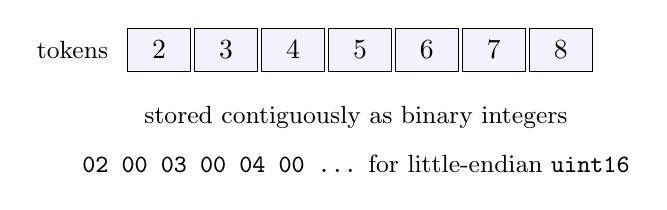
\begin{tikzpicture}[
  cell/.style={draw, minimum width=0.8cm, minimum height=0.55cm, align=center},
  lab/.style={font=\small, align=center}
]
\node[lab] at (-1.1,0) {tokens};
\foreach \i/\v in {0/2,1/3,2/4,3/5,4/6,5/7,6/8} {
  \node[cell, fill=blue!5] at (\i*0.85,0) {\v};
}
\node[lab] at (2.5,-0.85) {stored contiguously as binary integers};
\node[lab] at (2.5,-1.45) {\texttt{02 00 03 00 04 00 ...} for little-endian \texttt{uint16}};
\end{tikzpicture}
\end{center}

\subsection{Save And Load Code}

\begin{lstlisting}[language=Python]
import json
import numpy as np

def save_tokens(path, ids, dtype="uint16"):
    arr = np.array(ids, dtype=dtype)
    arr.tofile(path)

def load_tokens(path, dtype="uint16"):
    return np.fromfile(path, dtype=dtype)

def save_metadata(path, tokenizer_name, dtype, count, vocab_size):
    meta = {
        "tokenizer": tokenizer_name,
        "dtype": dtype,
        "count": int(count),
        "vocab_size": int(vocab_size),
        "byte_order": "little",
    }
    with open(path, "w") as f:
        json.dump(meta, f, indent=2)
\end{lstlisting}

\term{Why metadata matters}: \texttt{train.bin} alone is ambiguous. A future reader needs to know dtype, byte order, token count, tokenizer identity, and vocabulary size.

\section{Data Quality And Dataset Cards}

Data quality problems become model behavior problems. Before training, inspect:

\begin{itemize}
  \item duplicate documents;
  \item corrupted characters;
  \item broken markup;
  \item train/validation leakage;
  \item private or unsafe data;
  \item license restrictions;
  \item unexpected language mix;
  \item excessive boilerplate.
\end{itemize}

A dataset card should record:

\begin{longtable}{p{0.28\textwidth}p{0.54\textwidth}}
\toprule
\term{Field} & \term{Purpose} \\
\midrule
source & where the text came from \\
license & whether it can be used for training \\
preprocessing & normalization, filtering, deduplication \\
tokenizer & exact tokenizer name/version/hash \\
split & train, validation, test method \\
token count & number of tokens in each split \\
known risks & privacy, toxicity, quality, bias, leakage \\
checksums & reproducibility for final artifacts \\
\bottomrule
\end{longtable}

\engineering

Data code should be boring, explicit, and testable. A good data pipeline has:

\begin{lstlisting}
prepare script
tokenizer artifact
metadata JSON
binary token files
inspection tool
round-trip tests
train/valid split checks
\end{lstlisting}

The tokenizer is not a side file. It is part of the model's identity.

\labtitle{Build TinyGPT Token Data}

Use this mini-corpus:

\begin{lstlisting}
Tiny GPT models learn from tokens .
Tiny GPT models learn .
\end{lstlisting}

Use the TinyGPT vocabulary from this chapter.

\begin{enumerate}
  \item Encode each line as token IDs.
  \item Concatenate the lines into one token stream.
  \item With \(T=4\), build a window starting at position 0.
  \item Build a second window starting at position 3.
  \item State whether each window has enough tokens to form both \(x\) and \(y\).
\end{enumerate}

\section{Chapter Questions}

\begin{enumerate}
  \item Why does a GPT model need tokenization?
  \item What does \(V\) mean in the tokenizer/model contract?
  \item Why is changing the tokenizer dangerous for an existing checkpoint?
  \item What is the main weakness of character-level tokenization?
  \item What problem does subword tokenization solve?
  \item What does BPE merge during tokenizer training?
  \item Why does a training window need \(T+1\) tokens?
  \item What is train/validation leakage?
  \item Why store token streams in binary files?
  \item What metadata should accompany \texttt{train.bin}?
\end{enumerate}

\section{Solutions}

\begin{enumerate}
  \item A GPT model needs tokenization because neural networks operate on numerical tensors, not raw text. Tokenization maps text into integer IDs.

  \item \(V\) is vocabulary size. It is the number of distinct token IDs the model can read and predict. In TinyGPT, \(V=9\).

  \item Changing the tokenizer changes the meaning of token IDs. If ID \(2\) used to mean \texttt{Tiny} but later means something else, the learned embedding row 2 is misinterpreted.

  \item Character-level tokenization creates long sequences. Long sequences increase attention cost and make learning longer-range patterns harder.

  \item Subword tokenization handles rare or unseen words by splitting them into smaller known pieces while keeping common words or pieces compact.

  \item BPE merges frequent adjacent symbol pairs, such as \texttt{l} and \texttt{o} into \texttt{lo}, then possibly \texttt{lo} and \texttt{w} into \texttt{low}.

  \item A training window needs \(T+1\) tokens because \(T\) input positions require \(T\) next-token targets. The final input position needs one extra future token.

  \item Train/validation leakage happens when validation examples appear in training data. It makes validation metrics too optimistic.

  \item Binary files are compact and fast to read. They let training code stream large token arrays efficiently.

  \item Metadata should include tokenizer identity, dtype, token count, vocabulary size, byte order, split name, and ideally checksum/source information.
\end{enumerate}

\section{Lab Solution}

The first line:

\begin{quote}
\texttt{Tiny GPT models learn from tokens .}
\end{quote}

encodes as:

\[
[2,3,4,5,6,7,8].
\]

The second line:

\begin{quote}
\texttt{Tiny GPT models learn .}
\end{quote}

encodes as:

\[
[2,3,4,5,8].
\]

Concatenated stream:

\[
s=[2,3,4,5,6,7,8,2,3,4,5,8].
\]

With \(T=4\), a window starting at position 0 uses:

\[
\text{chunk}=[2,3,4,5,6].
\]

So:

\[
x=[2,3,4,5],
\qquad
y=[3,4,5,6].
\]

A window starting at position 3 uses:

\[
\text{chunk}=[5,6,7,8,2].
\]

So:

\[
x=[5,6,7,8],
\qquad
y=[6,7,8,2].
\]

Both windows have enough tokens because each has \(T+1=5\) tokens available.
